\documentclass[draftclsnofoot,onecolumn,10pt]{IEEEtran}
\usepackage[utf8]{inputenc}
\usepackage[margin=0.75in]{geometry}

\title{Auction Hunter \\ Technology Review Draft 1\\CS 461 - Fall 2018}
\author{Alexander Hull}
\date{October 11th, 2018}

\usepackage{cite}
\usepackage{graphicx}
\usepackage{setspace}
\usepackage{tabularx} % extra features for tabular environment
\usepackage{listings}
\usepackage{xcolor}

\colorlet{punct}{red!60!black}
\definecolor{background}{HTML}{EEEEEE}
\definecolor{delim}{RGB}{20,105,176}
\colorlet{numb}{magenta!60!black}


\lstdefinelanguage{json}{
    basicstyle=\normalfont\ttfamily,
    numbers=left,
    numberstyle=\scriptsize,
    stepnumber=1,
    numbersep=8pt,
    showstringspaces=false,
    breaklines=true,
    frame=lines,
    backgroundcolor=\color{background},
    literate=
     *{0}{{{\color{numb}0}}}{1}
      {1}{{{\color{numb}1}}}{1}
      {2}{{{\color{numb}2}}}{1}
      {3}{{{\color{numb}3}}}{1}
      {4}{{{\color{numb}4}}}{1}
      {5}{{{\color{numb}5}}}{1}
      {6}{{{\color{numb}6}}}{1}
      {7}{{{\color{numb}7}}}{1}
      {8}{{{\color{numb}8}}}{1}
      {9}{{{\color{numb}9}}}{1}
      {:}{{{\color{punct}{:}}}}{1}
      {,}{{{\color{punct}{,}}}}{1}
      {\{}{{{\color{delim}{\{}}}}{1}
      {\}}{{{\color{delim}{\}}}}}{1}
      {[}{{{\color{delim}{[}}}}{1}
      {]}{{{\color{delim}{]}}}}{1},
}


\begin{document}

\maketitle



\section{Abstract}
The components of our Auction Hunter program are: auction data source, auction database, and value calculation algorithms. We plan on acquiring real auction data from popular websites, storing them, performing value calculation, then displaying our results intelligently to the user. There are a plethora of tools that would be capable of completing this task, and this document will serve to discuss and compare options for each task. 

\newpage

\tableofcontents


\section{Introduction}
To intelligently select the right technology for the job, a number of factors must be considered: team combined experience, ease of use, compatibility with other tools, and supported features. The three components of our project that this document will cover are: Database tool, source of auction data, and auction ranking system. Our project needs to be able to pull data from any number of auction websites, then store that information in a database. Next, we need to perform calculations to determine which auction has the best value. 


\section{Database Management System}
 We will need to store the data acquired in a database. At its core, a database could be any organization of data. However, there are plenty of tools that abstract away the innards of the database and provide a logical interface. These pre-made tools will make our lives much easier, but not every database management system is treated equally.
 
\subsection{MongoDB}
MongoDB is a free, open source, and cross-platform database program. It is classified as  a document-oriented, NoSQL database. Document-oriented means that the data is stored in a format such as XML or JSON. NoSQL means it doesn't follow the conventional relational database functionality. A document-oriented database will likely be the best fit for our means, because it closely matches the format that we will be pulling data from. HTML is easily converted to JSON or XML. An example of what a JSON file might look like is available in Figure \ref{fig:xmlvshtml}. Additionally, there isn't a necessity to have a relational database because we only have a large collection of independent elements. MongoDB will be easy to learn and use because it is compatible with C++, Java, Python, and C\#. This means whatever language we choose to interface with, our data will be easily integrated into our database. After checking some of the documentation, it looks incredibly easy to get started with MongoDB. If using python, all that is required is a MongoDB install, import, then call MongoClient(). There is sample code for each language with snippets for simple tasks available on the MongoDB website. This could easily be added to our web crawling script to easily built up our database. It is open source so there is a plethora of documentation and other open source programs that use MongoDB.  \cite{MongoDB}

\begin{figure}[h]
\centering

\begin{lstlisting}[language=json,firstnumber=1]
{"car": {
  "vin": "1234567",
  "color": "Blue",
  "model": "ModelX"
}}

\end{lstlisting}
\caption{JSON example}
\label{fig:xmlvshtml}
\end{figure}



\subsection{Couch DB}
CouchDB is another open source, document-oriented database program. It is built to interface with JSON documents, which will be an advantage when capturing data from auctions. Unlike MongoDB, it takes a bit more work to interact with the database. To add to retrieve data, a program must make http requests (get, post, head, put). This means that any program that can create an HTTP request can interact with the database. However, it doesn't have some of the easy to use implementations built for specific languages. In terms of adding data, it is fairy intuitive . All a user would have to do is create a JSON structure for an entry, then make a POST request to the database. "Futon" is a built in administrative interface for displaying the database, which would be useful for development. It could be easier to develop and test our program if we can see the data being entered. \cite{CouchDB}

\subsection{MySQL}
MySQL is a widely used and well documented SQL database. Like MongoDB, it is easily integrated into languages such as python. MySQL has the advantage of using relational features such as keys. It seems that it would be easy to make an SQL call that simply selects all the cars that are white from our database. Finding a use for relationships might be difficult, because each car auction is an individual component. It could be useful if we eventually pull data from a wide array of sources, and we need to associate each auction with the original source. However, we don't necessary need to use the relational features that MySQL provides for it to fulfill all our requirements. As a consideration, the databases class at OSU uses MySQL to teach students. Therefore, our team would likely have the most combined experience working with SQL-like databases. \cite{mySQL}

\section{Auction Data Source}
 Each auction could be accessed conventionally with an internet browser, but we want to pull all the relevant information out automatically to avoid manually sifting through auctions. We will have to determine which website would provide the highest quantity of robust data.

\subsection{IAAI}
This website features IAA auctions for used and salvaged vehicles. We are focusing on Teslas, and there is a wide selection of auctions from around the United States. It is very easy to narrow your search based on a variety of parameters, which can be added to the URL. One great part about this website is it breaks down exactly what isn't working with the vehicle. If there is front end damage and the vehicle won't start, that will be specified on the auction page. It also displays which airbags were deployed, which greatly affects the value of the car. Figure \ref{fig:airbag} shows some of the information it provides. If we were to over simplify our backend algorithms, we could simply check the number of airbags deployed, and focus on vehicles that had only one deployed. This could give a user a rough estimate for the value of the auction. Ideally, our algorithm will be much more complicated than that, and the more data we have as input the better. Some other information that we can pull from each auction is: VIN, body style, make, model, damaged parts, condition, and lots of pictures of the vehicle. The website also has a current bid price, and time until bidding ends. Theoretically we could track the value of each vehicle, and if we find a vehicle is undervalued and reaching the final bid, we could automatically bid. Looking into the source of each page, it seems easy enough to filter out the relevant information, as it is displayed in the HTML file in an organized way, with relevant class names for each section. \cite{IAAI}

\begin{figure}[h]
\centering
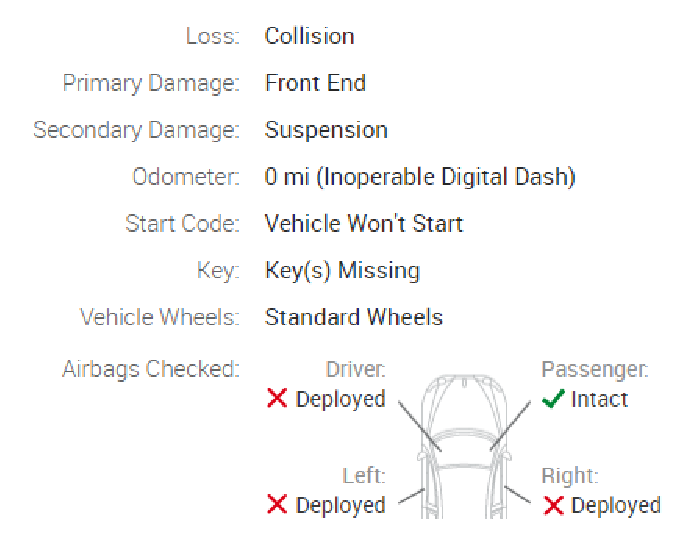
\includegraphics[scale=0.5]{airbag_capture}
\caption{Damage information on IAAI}
\label{fig:airbag}
\end{figure}


\subsection{Copart}
Copart is similar to IAAI, with slightly less damage information displayed. Other than that, it has all the similar search and filter features. The layout of the source is a bit more simple, which could make this a good website to start out with, as a proof of concept. There are uniform and high quality pictures of the vehicle that we could pull from the website. There is information about the current bid price, and the final sale date if it has been announced. In terms of the damage information, it has a text entry of the primary and secondary damage. The lack of airbag information is a large disadvantage. There are two similar models of Teslas listed, and the description of damage is the same but the actual damage is very different. One of the Teslas lists side damage, and has a big dent in the side. The other Tesla lists front end damage, and the entire front of the car is demolished. Unless a user evaluated the pictures for themselves, or a very advanced machine learning algorithm was used, these two auctions would be evaluated the same in the database. This website could be a good proof of concept website, and further development could combine multiple websites into one database. The one problem is we could find ourselves comparing lots of information to little, when comparing postings from different websites. \cite{copart}

\subsection{Auto Auction Mall}
Auto Auction Mall is similar to Copart because there is a somewhat limited amount of information. There is slightly less available information on this website. It simply displays where any primary damage is, and if the car starts or not. One advantage of this simplicity is it seems that there are only a few options for the car's status. With Copart, there was a text entry box where someone entering the information could be a bit more descriptive. Although there is more information available, it could be harder for a program to evaluate if it has to understand what the status means. A disadvantage of this website is it seems to rely heavily on JavaScript, meaning the layout of the HTML file is a bit harder to navigate, and could be difficult to pull information from. \cite{aam}

\section{Auction Ranking System Language}
Our value calculation could be performed with any turing complete programming language, but it is important to consider its compatibility with the other components. Ease of use and team experience are also important considerations. 

\subsection{Python}
Python has the benefit of easily integrating with many database options. For example, MySQL and MongoDB both have packages which you can include to make working with them very easy. Our group is all familiar working with python, so it should be easy for us to collaborate. Another benefit of using python is there are a number of easy packages to use for the web crawling. Whichever language we end up using for web crawling, we will likely end up using for the backend calculations. One language to interact with the whole backend process will be much easier to work with. Performance isn't much of a consideration for our purposes because we are working with relatively small sets of data, and will likely be bottlenecked by the speed of network connectivity rather than the program itself. 

\subsection{C++}
C++ is a favorable option because our team has a sufficient amount of combined experience working with th elanguage. It is moderately simple to get C++ to interface with our database system. However, it is nowhere near as easy when compared to python. C++ will be a good choice of language if we find ourselves doing some more heavy calculations on the data provided. Once the program has pulled all the relevant information out of the database, it will be easy in C++ to perform value calculations.  

\subsection{Java}
Java is somewhere in the middle between python and C++ when it comes to interfacing with a database such as MongoDB. Our group has the smallest combined experience in Java, but one member has comparable experience in Java as with C++. Java serves as a middle ground between C++ and python, and could be a compromise if some of our group prefers python and some prefer C++. 

\section{Conclusion}
After evaluating these possible technologies, there are clear advantages. MongoDB seems to be the easiest to use with Python. Getting it started is incredible simple, and the document oriented database is just what we need for lots of unrelated entries. The auction ranking language seems best suited for Python. Python is easy to use, but it also is great at interfacing with other programs, such as MongoDB or a web crawler. Additionally, our group has lots of experience working with Python. For the auction data source, IAAI seems to be the best pick. Although it is similar to Copart in terms of layout and design, it has much better damage information. Our algorithm is severely handicapped if it only has a couple parameters to base the evaluation on. Before a final decision is made, additional research, group approval, and cursory testing will be necessary. 


\bibliographystyle{IEEEtran}
\bibliography{IEEEabrv,bib}


\end{document}
